\documentclass[a4paper,11pt,onecolumn,twoside]{article}
\usepackage{fancyhdr}
\usepackage{threeparttable}
\usepackage{amsmath,amsfonts,amssymb}
\usepackage{graphicx}
\usepackage{fontspec}
\usepackage{booktabs}
\usepackage{indentfirst}
\usepackage{enumitem}
\usepackage{subcaption}
\usepackage{float}
\usepackage{bm}
\usepackage{caption}
\usepackage{graphicx}
% Please change the following fonts if they are not available.
\addtolength{\topmargin}{-54pt}
\setlength{\oddsidemargin}{-0.9cm}
\setlength{\evensidemargin}{\oddsidemargin}
\setlength{\textwidth}{17.00cm}
\setlength{\textheight}{24.50cm}
\usepackage{listings}
\usepackage{xcolor}
\usepackage[colorlinks,linkcolor=black,anchorcolor=black,citecolor=black]{hyperref}
\definecolor{dkgreen}{rgb}{0,0.6,0}
\definecolor{mauve}{rgb}{0.58,0,0.82}

\lstset{
	numbers=left,
	numberstyle=\tiny,
	stringstyle=\color{purple},
	basicstyle=\footnotesize\ttfamily, 
	keywordstyle=\color{blue}\bfseries,
	commentstyle=\color{olive},
	frame=shadowbox,
	%framerule=0pt,
	%backgroundcolor=\color{pink},
	rulesepcolor=\color{red!20!green!20!blue!20},
	%rulesepcolor=\color{brown}
	%xleftmargin=2em,xrightmargin=2em,aboveskip=1em
	escapeinside=``, 
	basicstyle=\tiny
}
\renewcommand{\baselinestretch}{1.1}
\parindent 22pt

\title{\Large \textbf{Analyzing the Dataset of Kobe Bryant Shot Selection}}
\author{
Mingyi Xue\footnote{Three authors are all exchange students from Nanjing University.}\\[2pt]
{\large \textit{School of Chemistry and Chemical Engineering, Nanjing University}}\\[6pt]Wangqian Miao
\\[2pt]
{\large \textit{Kuang Yaming Hornors School, Biophysics, Nanjing University}}\\[6pt]
Rui Wang\\[2pt]
{\large \textit{School of Business, Nanjing University}}\\[6pt]
\textbf{Instructor:} Prof. Cho-Jui Hsieh\\[2pt]
{\large \textit{Department of Computer Science \& Statistics, University of California, Davis}}\\[2pt]
}
\date{}

\fancypagestyle{firststyle}
{
   \fancyhf{}
   \fancyhead[C]{STA141C: High Performance Statistical Computing, Course Project}
   \fancyhead[R]{\thepage}
}

\pagestyle{fancy}
\fancyhf{}
\fancyhead[LE,RO]{\thepage}
\fancyhead[CE]{STA141C: High Performance Statistical Computing}
\fancyhead[RE]{}
\fancyhead[CO]{M. Xue, W. Miao, R. Wang: Analyzing the Dataset of Kobe Bryant Shot Selection }
\fancyhead[LO]{}
\setlist{nolistsep}
\captionsetup{font=small}
\newcommand{\supercite}[1]{\textsuperscript{\cite{#1}}}
\begin{document}
\maketitle
\thispagestyle{firststyle}
\setlength{\oddsidemargin}{ 1cm}
\setlength{\evensidemargin}{\oddsidemargin}
\setlength{\textwidth}{15.50cm}
\vspace{-.8cm}
\setcounter{page}{1}
\setlength{\oddsidemargin}{-.5cm}  % 3.17cm - 1 inch
\setlength{\evensidemargin}{\oddsidemargin}
\setlength{\textwidth}{17.00cm}

\begin{abstract}
In the real world application of machine learning, it is always difficult to apply the algorithms from books definitely. Most of the time, we find that our machine learning method does not work well without data pretreatment and feature engineering.\par 
Using 20 years of data on Kobe Bryant's swishes and misses in NBA, we will predict which shots can find the bottom of the net. By this dataset from Kaggle, we practice feature engineering with classification basic techniques like logistic regression , support vector machine and neural networks, and the up-to-date techniques like  XGBoost. At last, we give the conclusion of our job concretely.
\end{abstract}	
\section{Introduction}
When applying machine learning methods in the real world application, we always pretreat dataset, remove outliers, fill in missing values, create dummy variables, split dataset into train/dev/test sets and so on before we use the algorithms, especially in the case of that the dataset contains a lot of catogorical variables. However, nowadays, some algorithms can save us a lot time from feature engineering (for example, XGBoost method).\par
This dataset describes more than 30000 shots in Kobe's long career in Lakers, including different kinds of information about the shots and the game. Our task is to make the classification (the shot scores or not) as accurate as possible. In this paper, firstly, we transform the dataset into dataframe and then mine the most important information from the dataset through the plots. As a first try, we remove redundancy of multiple features to create a new dataset and then apply basic machine learning methods including logistic regression, SVM, neural networks on the set. Next, we tend to do more feature engineering with PCA and XGBoost to make our data matrix contain more accurate and focused infomation. At last, we will compare different algorithms on the updated data matrix.
\section{Data Summary and Data Preprocessing}
\subsection{Data Summary}
Kobe dataset has 30697 rows, 22 variables, among which \texttt{shot\_made\_flag} is the result whether he made the shot or not. Table 1 gives us a brief review of the features in our dataset. It is obvious that there exists so many catogorical variables in our dataset and that is why our task is so difficult.\par
\begin{table}[htbp]
	\centering
	\begin{tabular}{cccc}
		\midrule[1.5pt]
		\textbf{Name} &\textbf{Variable Kind}  &\textbf{Name}&\textbf{Variable Kind}\\
		\hline
	\texttt{action\_type} &category	&\texttt{seconds\_remaining}       &  int64			\\
    \texttt{combined\_shot\_type} &category	&\texttt{shot\_distance}     &   int64		\\
		\texttt{game\_event\_id}    &category	&\texttt{shot\_made\_flag}      			&response\\
		\texttt{game\_id}                     &category	&\texttt{shot\_type}                   &category	\\
		\texttt{lat}                         & float64	&\texttt{shot\_zone\_area}              &category		\\
		\texttt{loc\_x}                       &   int64&	\texttt{shot\_zone\_basic}             &category		\\
		\texttt{loc\_y}                       &   int64	&\texttt{shot\_zone\_range}             &category	\\
		\texttt{lon}                         & float64	&\texttt{team\_name}                   &category		\\
		\texttt{minutes\_remaining}           &   int64	&	\texttt{matchup}                     &category		\\
		\texttt{period}                      &   int64	&\texttt{opponent}                    &category		\\
		\texttt{playoffs}                    &category	&	
		\texttt{season}                      &category		\\	
		\midrule[1.5pt]
	\end{tabular}
	\caption{A summary table for the variables }
\end{table}
\par
There are 5000 rows with missing feature \texttt{shot\_made\_flag} because these rows are acted as test set on Kaggle competition. Since we needn't know the labels of these 5000 rows, we picked the rest 25697 rows and split them randomly into 70/30 as training set and test set.\par
At a glance of the dataset, it is easy to find that most of the variables are categorical, so we take a further step to see the number of categories in each variable and whether different categories have a significant effect on the average probability of $Y=1$ (Kobe made the shot) in Figure 1. Information on categorical variables are listed as follows.\par
\begin{table}[htbp]
	\centering
	\begin{tabular}{cccc}
		\midrule[1.5pt]
		\textbf{Name} &\textbf{Number of categories}&\textbf{Name}&\textbf{Number of categories}\\ 
		\hline
		\texttt{action$\_$type}				&57 &\texttt{shot$\_$zone$\_$area}		&6\\
		\texttt{shot$\_$zone$\_$basic}  		&7  &\texttt{opponent}    				&33\\
		\texttt{shot$\_$zone$\_$range}		&5& 
		\texttt{combined$\_$shot$\_$type}  &6\\          
		\texttt{team$\_$name} 				&1&
		\texttt{season}       				&20\\  
		\texttt{matchup}						&74&	\texttt{shot$\_$type} 				&2\\
		\midrule[1.5pt]
	\end{tabular}
	\caption{A summary table for the categorical variables }
\end{table}

\begin{figure}[htbp]
	\centering
	\begin{subfigure}[t]{0.30\textwidth}
		\centering
		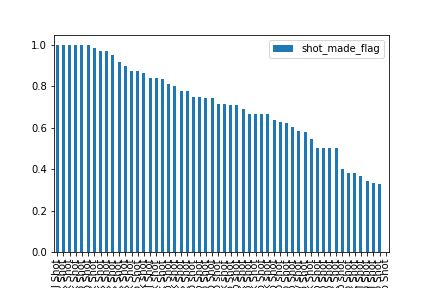
\includegraphics[width=1.0\textwidth]{action_type.png}
		\subcaption{action type}
	\end{subfigure}
	\quad
	\begin{subfigure}[t]{0.30\textwidth}
		\centering
		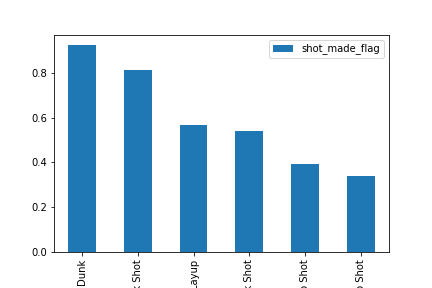
\includegraphics[width=1.0\textwidth]{combined_shot_type.png}
		\subcaption{combined shot type}
	\end{subfigure}	
	\quad
	\begin{subfigure}[t]{0.30\textwidth}
		\centering
		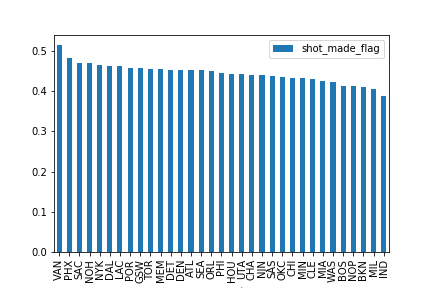
\includegraphics[width=1.0\textwidth]{opponent.png}
		\subcaption{opponent}
	\end{subfigure}	
	\\
	\begin{subfigure}[t]{0.30\textwidth}
		\centering
		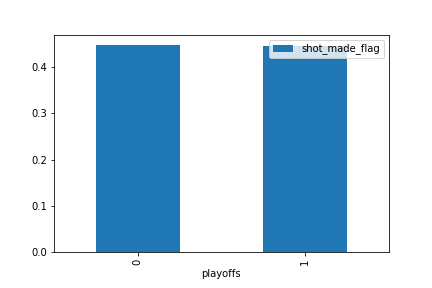
\includegraphics[width=1.0\textwidth]{playoffs.png}
		\subcaption{playoffs}
	\end{subfigure}
	\quad
	\begin{subfigure}[t]{0.30\textwidth}
		\centering
		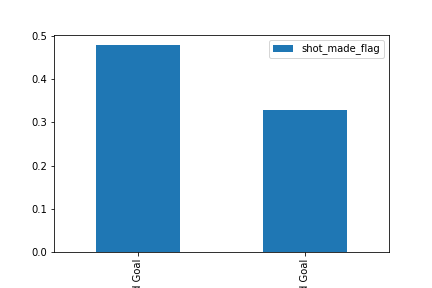
\includegraphics[width=1.0\textwidth]{shot_type.png}
		\subcaption{shot type}
	\end{subfigure}	
	\quad
	\begin{subfigure}[t]{0.30\textwidth}
		\centering
		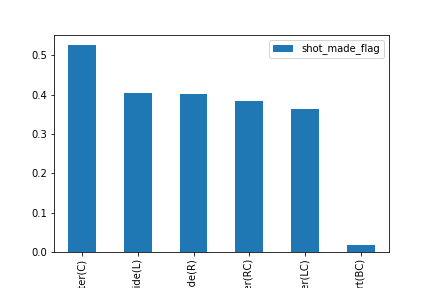
\includegraphics[width=1.0\textwidth]{shot_zone_area.png}
		\subcaption{shot zone area}
	\end{subfigure}	
	\\
	\begin{subfigure}[t]{0.30\textwidth}
		\centering
		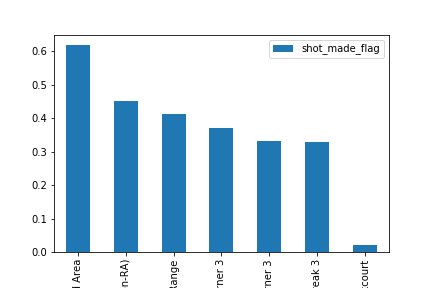
\includegraphics[width=1.0\textwidth]{shot_zone_basic.png}
		\subcaption{shot zone basic}
	\end{subfigure}	
	\quad
	\begin{subfigure}[t]{0.30\textwidth}
		\centering
		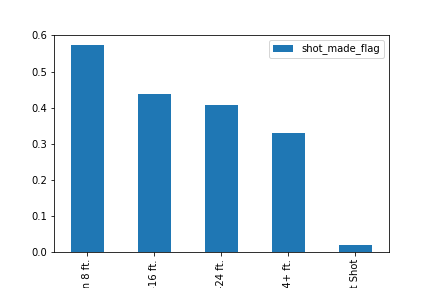
\includegraphics[width=1.0\textwidth]{shot_zone_range.png}
		\subcaption{shot zone range}
	\end{subfigure}	
	\quad
	\begin{subfigure}[t]{0.30\textwidth}
		\centering
		\subcaption*{}
	\end{subfigure}
	\caption{Barplots of mean value of categories}
\end{figure}
We can conclude from tables and plots above that the average probability of shot score varies in different categories and categories are in an acceptable number. So creating dummy variables (or one hot matrix) for each variable after feature engineering is doable.\par
\subsection{Data Preparation and Preprocessing}
In the firsthand, \texttt{shot\_id}, \texttt{game\_event\_id} and \texttt{game\_id} are all ordinal, subjective features created by people, so we removed them.\par
Secondly, we checked whether \texttt{lat/lon} contain almost the same infomation as \texttt{loc\_x/loc\_y} since they both recorded infomation on position.
\begin{figure}[htbp]
	\centering
	\begin{subfigure}[t]{0.45\textwidth}
		\centering
		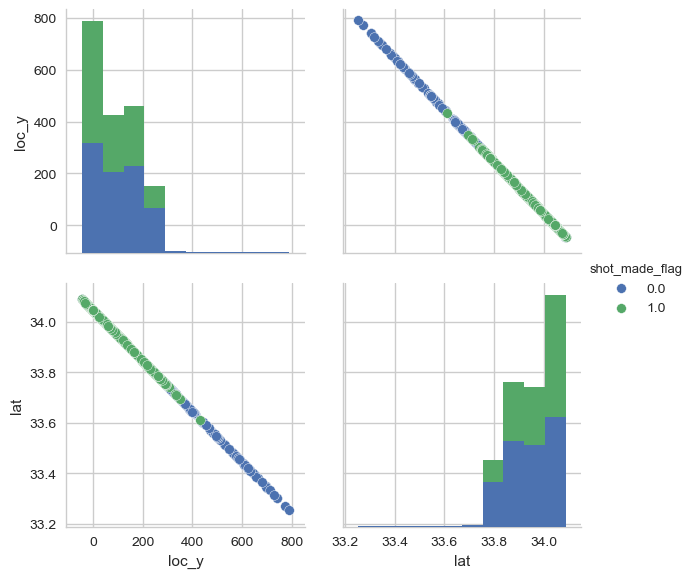
\includegraphics[width=1.0\textwidth]{lat_locy.png}
		\subcaption{Correlation between \texttt{lat} and \texttt{loc\_y}}
	\end{subfigure}
	\quad
	\begin{subfigure}[t]{0.45\textwidth}
		\centering
		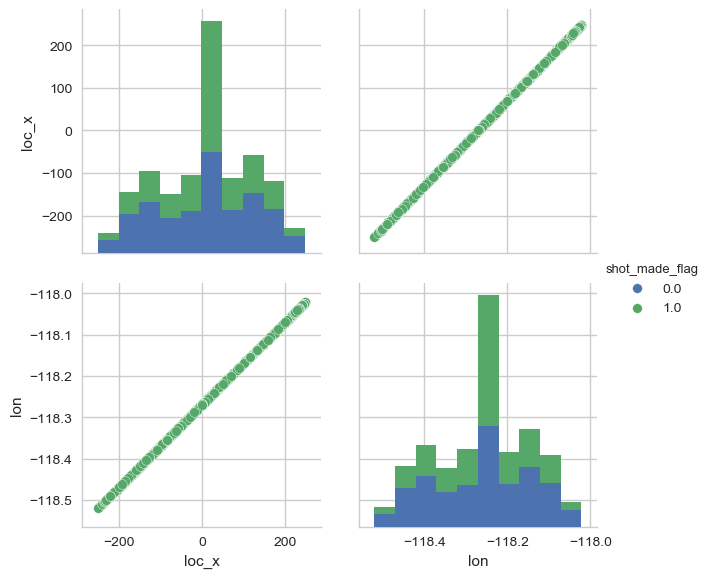
\includegraphics[width=1.0\textwidth]{lon_locx.png}
		\subcaption{Correlation between \texttt{lon} and \texttt{loc\_x}}
	\end{subfigure}	
\caption{Correlation between location and x,y}
\end{figure}
\par
It is obvious from the plot above that \texttt{lat} has a perfect negative linear relationship with \texttt{loc\_y} and \texttt{lon} has a perfect positive linear relationship with \texttt{loc\_x}, so we can remove features \texttt{lat} and \texttt{lon} from the dataset.\par
Then we noticed that game time both in large scale (date) or small scale (time) is an important factor in the dataset. In order to simplify data structure, we broke the feature \texttt{game\_date} into three orthogonal features \texttt{game\_year}, \texttt{game\_month} and \texttt{game\_day}. Besides, we combined \texttt{minutes\_remaining} and \texttt{seconds\_remaining} into \texttt{timeRemaining}.\par 
Furthermore, we plot the scatter plots to see how \texttt{loc\_x/loc\_y} can indicate zone features of the basketball field. It is safe to remove all indomation about zone, including \texttt{shot\_zone\_area}, \texttt{shot\_zone\_basic} and \texttt{shot\_zone\_range} according to the plot below.\par
\begin{figure}[htbp]
	\centering
	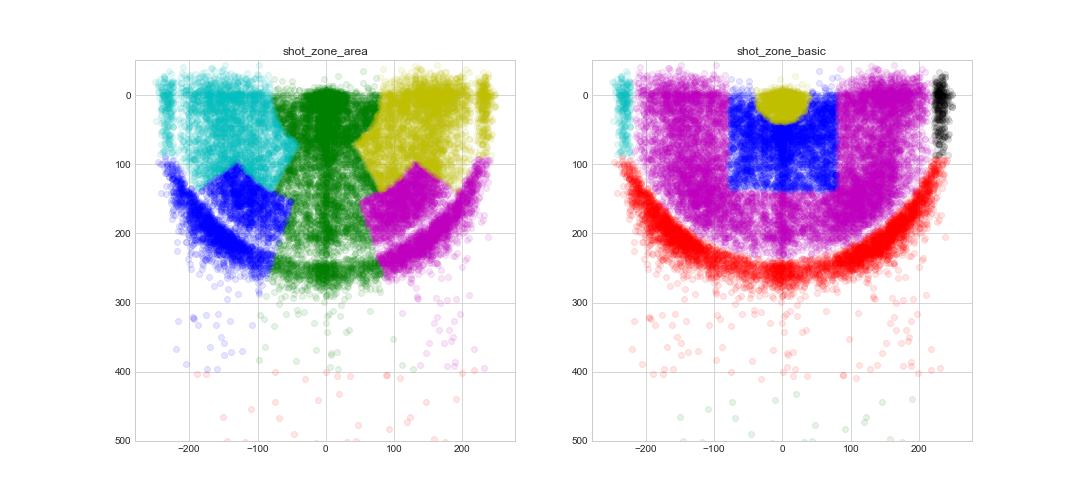
\includegraphics[width=1.0\textwidth]{shot_zone_plot.png}
	\caption{Plot of shot zones (different colors represent different regions)}
\end{figure}
Due to Kobe Bryant's staying in the same team for his all 20 years, we can remove \texttt{team\_id} and \texttt{team\_name} since these two features are consistent in the whole dataset.\par
Last but not least, it is interesting to find that matchup contains the infomation of opponent but more than that. We broke \texttt{matchup} down to \texttt{opponent} and \texttt{homeGame}, which indicate whether a game is hosted at home or away.\par 
In conclusion, we created dummy variables for all categorical features and got totally 117 features including labels of \texttt{shot\_made\_flag}.
\section{Basic Supervised Learning Methods}
After we clean the data and do the basic preprocessing, we will apply some basic classification algorithms. In this section, the behaviour of logistic regression, Support Vector Machine and Neural Networks will be discussed when we choose different parameters, kernel functions, and depth of our Nerual Networks.
\subsection{Logistic Regression}
Firstly, Logistic Regression is the basic classification algorithm in machine learning, especially useful for binomial classification.  We try to find a linear relationship between logit($\pi$) and explanatory variables, where logit($\pi$) $= \ln(\frac{\pi}{1-\pi})$ and $\pi$ is the probability of $Y=1$.
\par
In Logistic Regression, there are several important parameters such as how we choose the cutoff value (in common, we choose 0.5 to tell the difference between 0 and 1), the regularization term and the parameters for the regularization term.\par 
The value of cutoff is quite significant when we use logistic regression. Different cutoffs will give us different error matrixes. As shown in Figure 4, authors find the best cutoff is 0.55.\par 
We fixed the cutoff value and changed the hyperparameters for the regularization term in this problem. Results are as follows.
\begin{table}[htbp]
	\centering
	\begin{threeparttable}[b]
	\begin{tabular}{ccccc}
		\midrule[1.5pt]
	\textbf{Cutoff Value} &\textbf{Regularization}  &\textbf{$\lambda$}&\textbf{Train Accuracy}&\textbf{Test Accuracy}\\
		\hline
		0.50\tnote{1}&$\ell_2$&1.0&44.65\%&44.47\% \\
		0.55\tnote{2}&$\ell_2$&1.0&68.35\%&68.50\%\\
		0.55&$\ell_2$&10.0&63.44\%&64.10\%\\
		0.55&$\ell_1$&1.0&67.43\%&66.43\%\\
		\midrule[1.5pt]
	\end{tabular}
	\begin{tablenotes}
		\item [1] Implemented by authors
		\item [2] Implemented with \texttt{sklearn.linear\_model.LogisticRegression}
	\end{tablenotes}
	\end{threeparttable}
\caption{Table for Logistic Regression behaviour}
\end{table}
\begin{figure}[htbp]
	\centering
	\begin{subfigure}[t]{0.45\textwidth}
		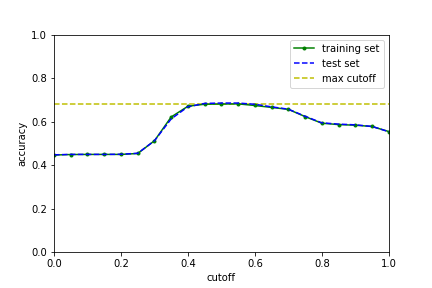
\includegraphics[width=1.0\textwidth]{logistic_cutoff.png}
		\subcaption{Plot of accuracy vs. cutoff}
	\end{subfigure}
	\quad
	\begin{subfigure}[t]{0.45\textwidth}
		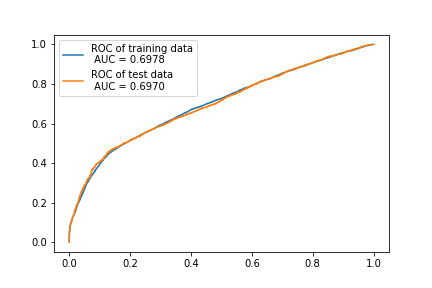
\includegraphics[width=1.0\textwidth]{logistic_ROC.png}
		\subcaption{ROC}
	\end{subfigure}
\caption{The behaviour of Logistic Regression}
\end{figure}
\par
From the experiment above we had some basic observation as following.
\begin{itemize}
	\item The cutoff value will significantly influence the behaviour of Logistic Regression and in this expriment, the best cutoff is 0.55. However, there may be overfitting because the test accuracy is higher than train accuracy. 
	\item $\ell_2$ regularization and $\lambda=1$ is a good choice for this problem.
	\item AUC is between $(0.60, 0.70)$ and the Logistic Regression model is moderately fit for this task.
\end{itemize}
\subsection{Support Vector Machine}
SVM is a fast and dependable classification algorithm that performs very well with a limited amount of data and that is why we choose it as our second algorithm.\par
In this task we just ran different kernel functions with the help of sklearn  due to the authors are not familiar with the SVM algorithm (We just use SVM for reference) and test the performance of SVM on our dataset. The results are shown in Table 4.\par 
It is obvious that the linear kernel gives us the best results which is close to the accuracy of Logistic Regression.
\begin{table}[htbp]
	\centering
	\begin{tabular}{cccc}
		\midrule[1.5pt]
	\textbf{Kernel} &\textbf{Time consuming}(s)  &\textbf{Train Accuracy}&\textbf{Test accuracy}\\
		\hline
		\texttt{rbf}&91.83&67.30\%&67.98\%\\
		\texttt{linear}&74.96&68.07\%&68.46\%\\
		\texttt{poly}&85.56&55.40\%&55.31\%\\
		\midrule[1.5pt]
	\end{tabular}
	\caption{Table for SVM behaviour}
\end{table}
\subsection{Neural Networks}
Nowadays, Neural Network is a popular way to realize classification, especially in computer vision. In this task, we hope to use Neural Networks to find whether there exists some non-linear pattern in our data. \par 
With the help of tensorflow, we can build our own neural networks easily. However, so many hyperparameters exist in neural networks, like learning rate, mini-batch size, number of layers and neurons in each layer, activation fuction and so on. We do some tests to see how they will affect our models' behaviour.\par
In this problem, we firstly transform the 0/1 label to one hot matrix. We applied ReLU to hidden layers and softmax to output layers. Mini-batch size equals the whole dataset which means we used normal gradient descent algorithm, and the initial learning rate (denoted as $\alpha$) is 0.1.
\begin{table}[H]
	\centering
	\begin{tabular}{cccccc}
		\midrule[1.5pt]
		\textbf{Depth} &\textbf{Neurons}&\textbf{iterations}  &\textbf{decrease in $\alpha$}&\textbf{Train Accuracy}&\textbf{Test Accuracy}\\
		\hline
		3&[25,12,2]&10000&no&69.83\%&65.84\%\\
		3&[25,12,2]&10000&yes&69.18\%&68.65\%\\
		5&[32,16,8,4,2]&5000&yes&69.00\%&67.84\%\\
		\midrule[1.5pt]
	\end{tabular}
	\caption{Table for Neural Networks behaviour}
\end{table}
\begin{figure}[htbp]
	\centering
	\begin{subfigure}[t]{0.31\textwidth}
		\centering
		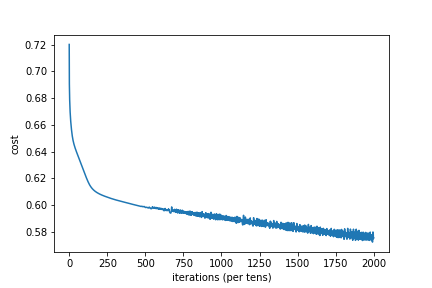
\includegraphics[width=1.0\textwidth,height=0.18\textheight]{nn3_10000_no.png}
		\subcaption{No decrease in $\alpha$}
	\end{subfigure}
	\quad
	\begin{subfigure}[t]{0.31\textwidth}
		\centering
		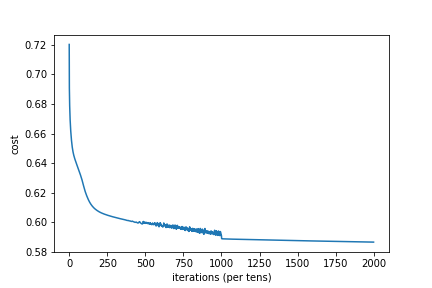
\includegraphics[width=1.0\textwidth,height=0.18\textheight]{nn3_10000.png}
		\subcaption{$\alpha \times 0.1$ every 5000 iteration}
	\end{subfigure}	
	\quad
	\begin{subfigure}[t]{0.31\textwidth}
		\centering
		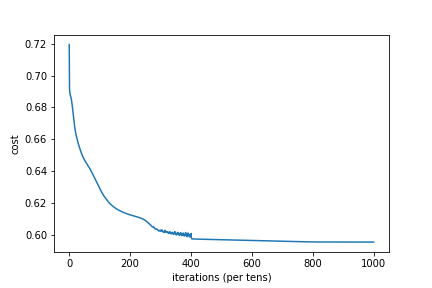
\includegraphics[width=1.0\textwidth,height=0.18\textheight]{nn5_5000.png}
		\subcaption{$\alpha \times 0.1$ every 2000 iteration}
	\end{subfigure}	
	\caption{Importance of decrease in learning rate }
\end{figure}
\par
Here are several findings.
\begin{itemize}
	\item A decrease in learning rate is important in neural network because large steps will lead to increasing oscillation as iteration goes on.
	\item For this dataset, since the amount of data is not large enough, there seems no significant difference in training effects for shallow or deep neural networks. 
	\item Usually deeper neural networks need more time to complete each iteration (That's why our attempt to train a 10-layer neural network failed due to limited time and computing resources).
	\item  We prefer to train the 3-layer network with more iterations to reach higher accuracy in a shoter time. 
\end{itemize}
\subsection{Algorithm Comparison}
As shown above, we applied three different classification algorithms. In Table 6, we comprare the model performace of them.
\begin{table}[htbp]
	\centering
	\begin{tabular}{cccc}
		\midrule[1.5pt]
		\textbf{Algorithm} &\textbf{Time consuming}(s)  &\textbf{Train Accuracy}&\textbf{Test Accuracy}\\
		\hline
		Logistic Regression&0.5305&68.35\%&68.50\%\\
		SVM  &74.96&68.07\%&68.46\%\\
		Neural Networks&1183.87&69.18\%&68.65\%\\
		\midrule[1.5pt]
	\end{tabular}
	\caption{Algorithms compaison}
\end{table}
\par The conclusion is as following.
\begin{itemize}
	\item Three different methods give us almost the same accuracy.
	\item Neural Networks take much more time than other algorithms.
	\item It seems that the non-linear pattern in our data is not obvious.
\end{itemize}
\section{Dimension Reduction and Feature Engineering}
Now, our dataset contains 117 features (including dummy variables) which may contain some trivial information, for example, some categories just have a couple rows and the truth is that the data matrix is a large sparce matrix (We have so many dummy variables). Dimension reduction or important feature selection may help us know more about the most important features in the dataset. In this section, we apply PCA which is unsupervised and XGBoost which is supervised to deal with the problem. 
\subsection{Dimension Reduction with PCA}
Principal Component Analysis (PCA) is a statistical procedure that extracts the most important features of a dataset.\par
Firstly, we normalized each column of the 117-feature dataset to mean 0, standard deviation of 1 normal distribution by $\frac{X-\bar{X}}{SE\{X\}}$. Then we computed the correlation matrix of the normalized dataset which is denoted as $\bm{C}$. Furthermore, we applied sklearn.decomposition.PCA on the matrix $\bm{C}$ to find columns in the normalized data which can explain 99.9\% of the total variance. Finally, 4 columns remained as the compacted dataset and we applied the same classification algorithm discussioned above on it.
\begin{table}[H]
	\centering
	\begin{tabular}{cccc}
		\midrule[1.5pt]
		\textbf{Algorithm} &\textbf{Time consuming}(s)  &\textbf{Train Accuracy}&\textbf{Test Accuracy}\\
		\hline
		Logistic Regression&--&--&57.78\%\\
		SVM  &86.74&--&59.88\%\\
		Neural Networks&468.92&60.48\%&60.11\%\\
		\midrule[1.5pt]
	\end{tabular}
	\caption{Algorithms comparisons after PCA}
\end{table}
\begin{itemize}
	\item Though the accuracy of compacted data is around 60\%, which is a little far away from the accuracy of 68\% of the whole dataset, taking the fact of only 4 columns into consideration, these columns have contributed to half of the probability gain in prediction compared to the 50\% probability abtained by guessing based on a coin-flip. 
	\item PCA is efficient in data compact, but there is still a problem in this project that most of the variables are dummy variables which is binomially distributed and cannot be normalized in the same way as numeric variables. Instead, standardized pearson residuals are recmmended for those dummy variables.
\end{itemize}
\subsection{Feature Engineering with XGBoost}
XGBoost is short for ``Extreme Gradient Boosting”, where the term ``Gradient Boosting” is proposed in the paper Greedy Function Approximation: A Gradient Boosting Machine, by Friedman.  XGBoost is based on this original model which is applied by many data scientists in Kaggle to realize feature engineering. XGBoost is an ensemble method and realized by C++ and OpenMP. We get the final results with 4 thread and 500 iterations in just few seconds.\par 
Through XGBoost, we can find the interesting features in our dataset as shown in the following figure and then pick them up to make our model more specific and accurate.
\begin{figure}[htbp]
	\centering
	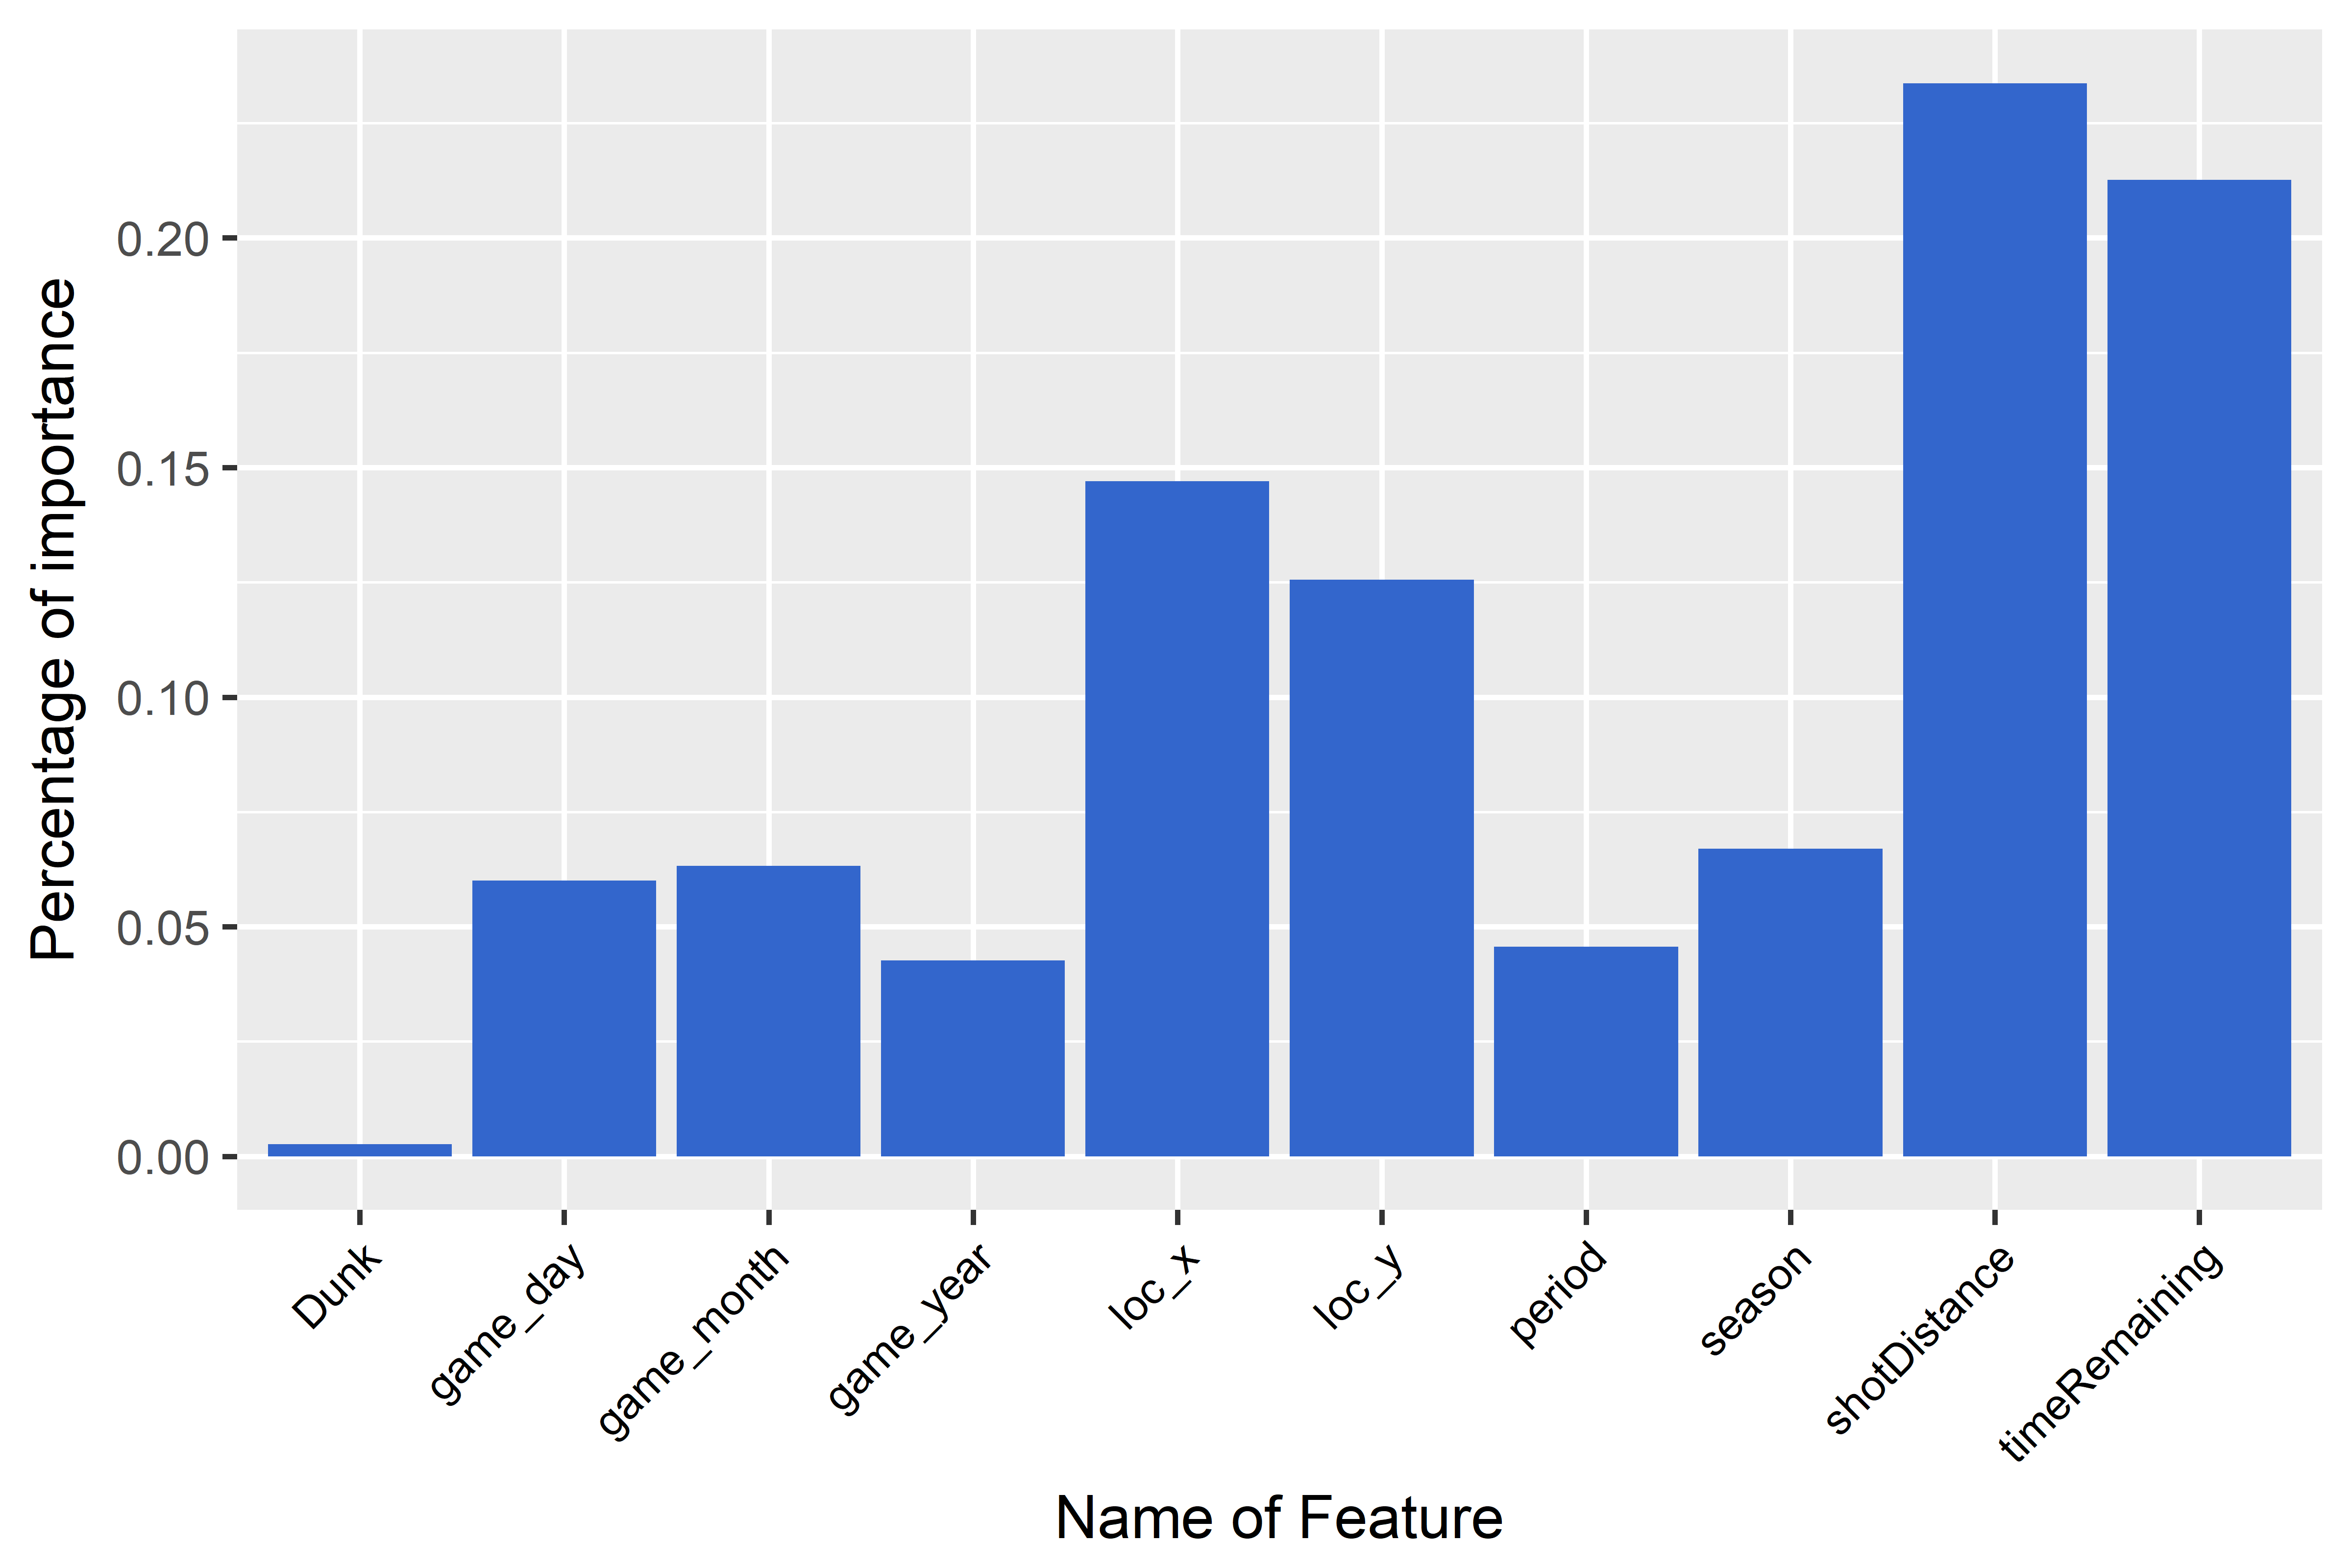
\includegraphics[width=0.8\textwidth]{important_features.png}
	\caption{Ten most important features}
\end{figure}
\par XGBoost gives us a more smaller and denser data matrix and we applied the algorithms on the new dataset again, as shown in Table 8. It seems that the 10 most important features explains the most important behaviour of our dataset.
\begin{table}[H]
	\centering
	\begin{tabular}{cccc}
		\midrule[1.5pt]
		\textbf{Algorithm} &\textbf{Time consuming}(s) &\textbf{Train Accuracy} &\textbf{Test Accuracy}\\
		\hline
		Logistic Regression&0.2325&60.32\%&61.23\%\\
		SVM  &19.22&58.90\%&58.91\%\\
		Neural Networks&273.42&60.41\%&60.92\%\\
		\midrule[1.5pt]
	\end{tabular}
	\caption{Algorithms comparison  after XGBoost}
\end{table}
\section{Conclusion}
One important characteristic of our dataset is that the amount of data is not big enough to behave differently with diffenrent classification algorithms. That's a major reason of why logistic regression sometimes even works better than neural networks and why XGBoost does not seem to revolutionize prediction of the dataset a lot.\par
We suppose to get vote results from three basic classification prediction and expect to see an improvement in accuracy as a followup step.
\section{Acknowledgement}
This work is supervised by Prof. Cho-Jui Hsieh who gives us a bunch of useful advice. The authors learn a lot from the following websites and tutorials. Without these generous people, we cannot finish this difficult job. Thanks a lot!
\begin{enumerate}
	\item Prof. Cho-Jui Hsieh's lecture notes on STA141C.
 	\item Andrew Ng's course on Coursera: Deep Learning Specialization.
	\item Scikit-learn tutorial: \url{http://scikit-learn.org/stable/documentation.html}.
	\item Kaggle competition discussion: \url{https://www.kaggle.com/c/kobe-bryant-shot-selection}.
	\item XGBoost tutorial: \url{https://xgboost.readthedocs.io/en/latest/R-package/index.html}.
\end{enumerate}
\end{document}
